

\begin{figure}[H]
	\centering
	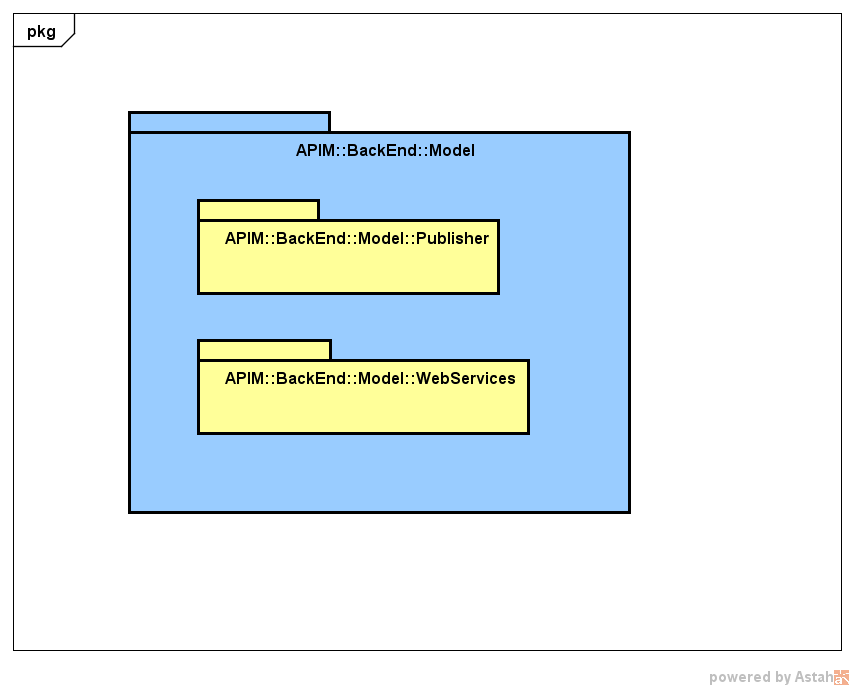
\includegraphics
	[width=0.7\linewidth]
	{UML/DiagrammiPackage/Model.png}
	\caption{Package APIM::BackEnd::Model}
\end{figure}

Il package \textit{Model} contiene i packages utilizzati per rappresentare i dati e l'implementazione della logica di business e di validazione.
\begin{itemize}
	\item \textbf{Publisher}: contiene le classi per la pubblicazione dei dati;
	\item \textbf{WebServices}: contiene le classi per la comunicazione col database.
\end{itemize}


\subsubsection{Publisher}
\begin{figure}[H]
	\centering
	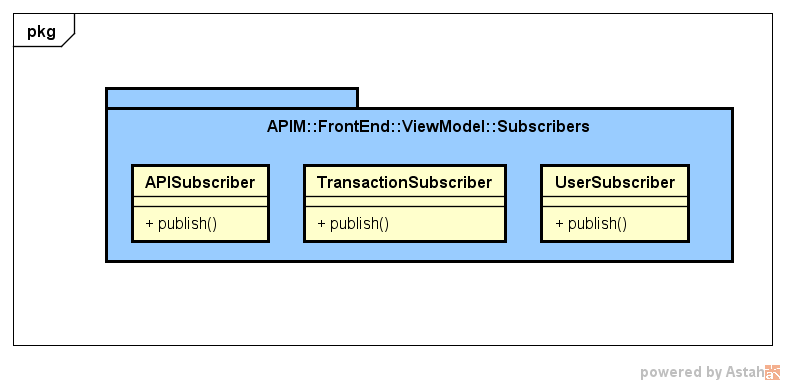
\includegraphics
	[width=0.7\linewidth]
	{UML/DiagrammiPackage/Publisher.png}
	\caption{Package APIM::BackEnd::Model::Publisher}
\end{figure}

Il package \textit{Publisher} contiene le classi necessarie ad esporre il modello dati al front-end.

\paragraph{APIPublisher}
\begin{itemize}
	\item \textbf{Funzione del componente}: esegue la pubblicazione delle API;
	\item \textbf{Attivita’ svolte e dati trattati}: permette l'accesso alla collezione di API.
\end{itemize}

\paragraph{TransactionPublisher}
\begin{itemize}
	\item \textbf{Funzione del componente}: esegue la pubblicazione delle transazioni;
	\item \textbf{Attivita’ svolte e dati trattati}: permette l'accesso alla collezione di transazioni.
\end{itemize}

\paragraph{UserPublisher}
\begin{itemize}
	\item \textbf{Funzione del componente}: esegue la pubblicazione degli utenti;
	\item \textbf{Attivita’ svolte e dati trattati}: permette l'accesso alla collezione di utenti.
\end{itemize}


\subsubsection{WebServices}

\begin{figure}[H]
	\centering
	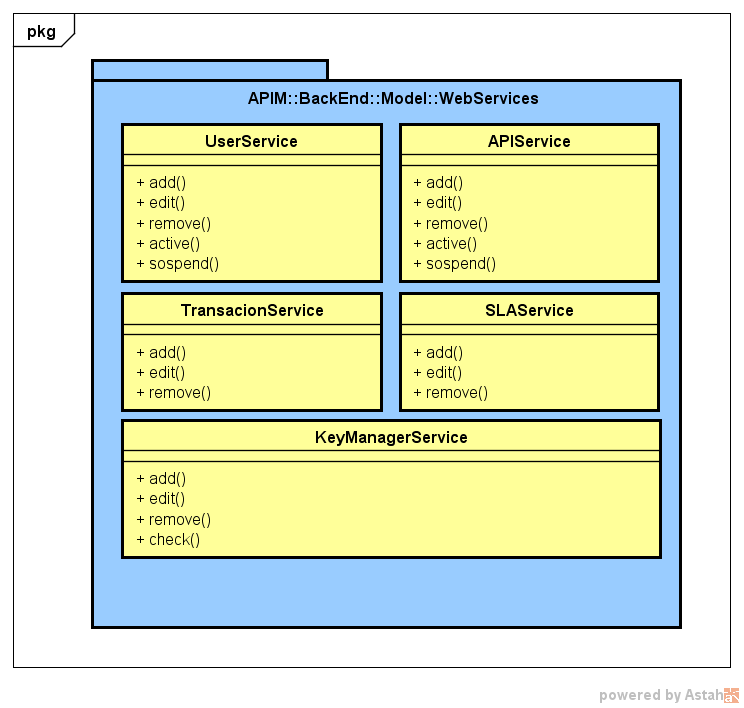
\includegraphics
	[width=0.7\linewidth]
	{UML/DiagrammiPackage/WebServices.png}
	\caption{Package APIM::BackEnd::Model::WebServices}
\end{figure}

Il package \textit{WebServices} contiene i microservizi utilizzati per mettere in comunicazione il database con il \textit{Model}.

\paragraph{UserService}
\begin{itemize}
	\item \textbf{Funzione del componente}: esegue le funzioni di inserimento, modifica e rimozione di utenti;
	\item \textbf{Relazioni d’uso di altri componenti}: si interfaccia con la \textit{ViewModel} e il database per fornire le funzioni di inserimento, modifica e rimozione di utenti.
\end{itemize}

\paragraph{APIService}
\begin{itemize}
	\item \textbf{Funzione del componente}: esegue le funzioni di inserimento, modifica e rimozione di API;
	\item \textbf{Relazioni d’uso di altri componenti}: si interfaccia con la \textit{ViewModel} e il database per fornire le funzioni di inserimento, modifica e rimozione di API.
\end{itemize}

\paragraph{TransactionService}
\begin{itemize}
	\item \textbf{Funzione del componente}: esegue le funzioni di inserimento, modifica e rimozione di transazioni;
	\item \textbf{Relazioni d’uso di altri componenti}: si interfaccia con la \textit{ViewModel} e il database per fornire le funzioni di inserimento, modifica e rimozione di transazioni.
\end{itemize}


\paragraph{SLAService}
\begin{itemize}
	\item \textbf{Funzione del componente}: esegue le funzioni di inserimento, modifica e rimozione di log di SLA;
	\item \textbf{Relazioni d’uso di altri componenti}: si interfaccia con la \textit{ViewModel} e il database per fornire le funzioni di inserimento, modifica e rimozione di log di SLA.
\end{itemize}

\paragraph{KeyManagerService}
\begin{itemize}
	\item \textbf{Funzione del componente}: esegue le funzioni di inserimento, modifica e rimozione di API key;
	\item \textbf{Relazioni d’uso di altri componenti}: si interfaccia con la \textit{ViewModel} e il database per fornire le funzioni di inserimento, modifica e rimozione di API key.
\end{itemize}

